\begin{figure}[t]
\centering
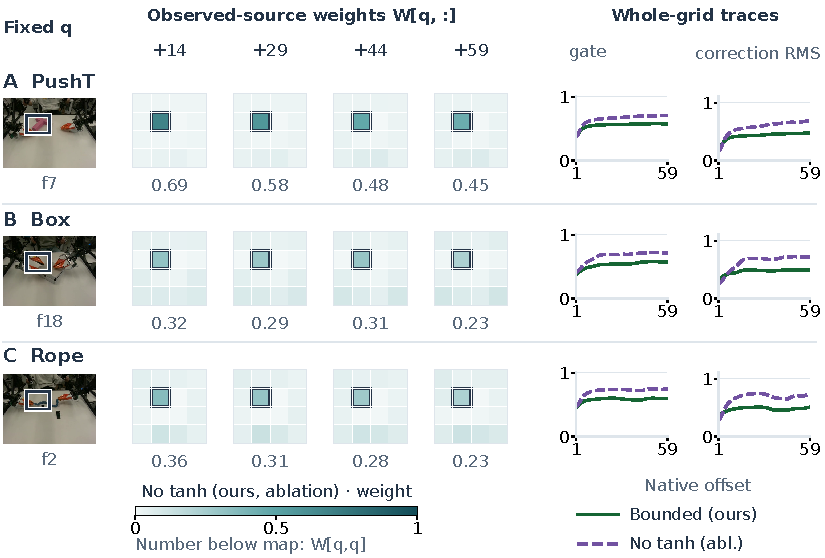
\includegraphics[width=\linewidth]{generated/qualitative_temporal_v1/temporal_decoder.pdf}
\caption{\textbf{Reading a fixed observation across forecast steps.}
The cases and offsets match Figure~\ref{fig:temporal-qualitative-outcomes}.
Left: the observed frame marks a fixed query coordinate $q$ (row 2, column 2);
the marker identifies a feature-grid coordinate, not a localized object.
Center: the no-$\tanh$ ablation's effective weights $W_h[q,:]$ over all 16
\emph{observed} source locations, on a shared $[0,1]$ scale. The outlined cell
is the same-location source; its weight is printed below each map.
Right: bounded/no-$\tanh$ trajectories of the mean gate and correction RMS.
These summaries cover the \emph{whole grid}, not only $q$; correction RMS is
computed over $16\!\times\!384$ coordinates separately per seed.
We average each seed's weights and diagnostics only after their nonlinear
operations. These are measured feature-mixing diagnostics, not semantic
attention or causal attribution. RMS values use task-specific standardization.
Future photographs are never added to memory.
Recorded scenes: RLA-WM/IWS dataset.}
\label{fig:closest-decoder-internals}
\end{figure}
